\documentclass[12pt]{article}

\usepackage[utf8x]{inputenc} % Включаем поддержку UTF8  
\usepackage[russian]{babel}  % Включаем пакет для поддержки русского языка  
\usepackage{hyperref}        % Для гиперссылок

% Математика
\usepackage{amsmath}         % В т.ч. для матриц
\usepackage{amssymb}

% Прога
\usepackage{etoolbox}
\usepackage{listings}

% Цвета
\usepackage{xcolor}

% Картинки
\usepackage{graphicx}
\graphicspath{ {./images/} }

\newtheorem{property}{Свойство}
\newtheorem{consequence}{Следствие}[property]

\newcommand{\qedsymbol}{\rule{2mm}{2mm}}

\begin{document}

\thispagestyle{empty}
\begin{center}
\textbf{ПРАВИТЕЛЬСТВО РОССИЙСКОЙ ФЕДЕРАЦИИ}

\vspace{5ex}
	
\textbf{Федеральное государственное автономное образовательное учреждение \\ высшего образования \\ <<Национальный исследовательский университет \\ <<Высшая школа экономики>>}
\end{center}
\vspace{5ex}

\begin{center}
    Московский институт электроники и математики им. А.Н. Тихонова  
    
    \vspace{5ex}
    
    Департамент прикладной математики
    
    \vspace{10ex}
    \textbf{Отчёт \\ по лабораторной работе №2 \\ по курсу <<Алгоритмизация и программирование>>}
	\vspace{7ex}

\end{center}

\begin{center} 
\begin{tabular}{| p{0.3\linewidth}| p{0.3\linewidth}| p{0.3\linewidth}|}
 \hline	
ФИО студента & Номер группы & Дата \\  \hline
 & & \\  
Вязов Глеб \newline Дмитриевич & БПМ-231 & 22.10.2023\\  
 & & \\  \hline		
\end{tabular}
\end{center}

\begin{center}
	\vspace{3ex}
	
	\vfill
   
   \normalsize
    
	\textbf{Москва, 2023}
\end{center}

\newpage

%---------------------------------------------------------------------------------

\section*{Задание (вариант №7)}
Даны числа x и y. Определить, принадлежит ли точка с координатами (x, y) заштрихованной области, включая границы.

Оформить первое решение в виде вложенных условных операторов с простыми условиями.

Второе решение должно содержать один условный оператор со сложным логическим условием.

Третье решение должно быть оформлено в виде отдельной функции, вызываемой из основной программы. Функция не содержит условного оператора, а только логическое выражение.

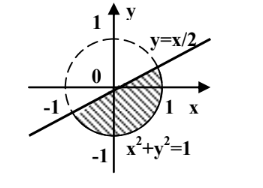
\includegraphics{img1}

\newpage

%---------------------------------------------------------------------------------

\section*{Решение}\addcontentsline{toc}{section}{Решение}

\lstset{ %
texcl=true,%
language=C,                 % выбор языка для подсветки
basicstyle=\small\sffamily, % размер и начертание шрифта для подсветки кода
numbers=left,               % где поставить нумерацию строк (слева\справа)
numberstyle=\tiny,           % размер шрифта для номеров строк
stepnumber=1,                   % размер шага между двумя номерами строк
numbersep=5pt,                % как далеко отстоят номера строк от подсвечиваемого кода
backgroundcolor=\color{white}, % цвет фона подсветки - используем \usepackage{color}
showspaces=false,            % показывать или нет пробелы специальными отступами
showstringspaces=false,      % показывать или нет пробелы в строках
showtabs=false,             % показывать или нет табуляцию в строках
frame=single,              % рисовать рамку вокруг кода
tabsize=3,                 % размер табуляции по умолчанию равен 2 пробелам
captionpos=t,              % позиция заголовка вверху [t] или внизу [b] 
breaklines=true,           % автоматически переносить строки (да\нет)
breakatwhitespace=false, % переносить строки только если есть пробел
escapeinside={\%*}{*)},   % если нужно добавить комментарии в коде
inputencoding=utf8x,
extendedchars=\true
}

\begin{lstlisting}[label=string_code1,caption=C]
#include <stdio.h>

int isBelongs(double x, double y) {
    return (y < x / 2.0 && x*x + y*y <= 1) || (y == x / 2.0);
}

int main() {
    // Меняем кодировку на UTF-8, чтобы можно было писать на русском
    system("chcp 65001");

    double x, y;

    // Ввод переменных. Дружественный интерфейс
    printf("Выполнил задание: Вязов Глеб. Группа: БПМ231\n");
    printf("Введите значение x (дробное): ");
    scanf("%lf", &x);
    printf("Введите значение y (дробное): ");
    scanf("%lf", &y);

    // 1 способ
    if (y == x / 2.0) {
        printf("ДА");
    } else if (y < x / 2.0) {
        if (x*x + y*y <= 1) {
            printf("ДА");
        } else {
            printf("НЕТ");
        }
    } else {
        printf("НЕТ");
    }
    printf("\n");

    // 2 способ
    if ((y < x / 2.0 && x*x + y*y <= 1)
        || (y == x / 2.0)) {
        printf("ДА");
    } else {
        printf("НЕТ");
    }
    printf("\n");

    // 3 способ
    if (isBelongs(x, y)) {
        printf("ДА");
    } else {
        printf("НЕТ");
    }

    return 0;
}
\end{lstlisting} 

\newpage

%---------------------------------------------------------------------------------

\section*{Тестирование}

\begin{enumerate}

\item \textbf{Тест №1.} 

\textit{Ввод:} 1, 1

\textit{Вывод:} 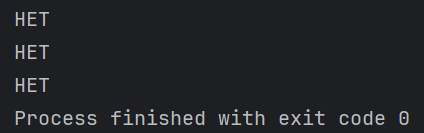
\includegraphics{img2}



\item \textbf{Тест №2.}

\textit{Ввод:} -1, -1

\textit{Вывод:} 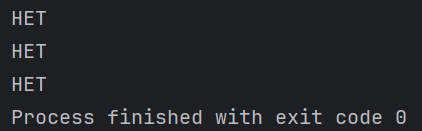
\includegraphics{img3}



\item \textbf{Тест №3.}

\textit{Ввод:} 0.5, 0.2

\textit{Вывод:} 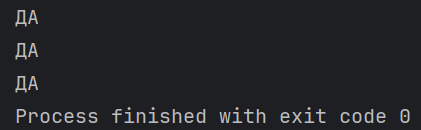
\includegraphics{img4}



\end{enumerate}


\end{document}
